\section{Typed realizability}
\label{sec:typed-realizability}

RZ is based on \emph{typed realizability} by John
Longley~\cite{Longley99}. It is a variant of realizability that most
directly corresponds to the informal view that a programmer has in
mind when thinking about an implementation of a structure.

We motivate and explain typed realizability and its relationship with
real-world programming by way of example. Suppose we are asked to
design a data structure for the set $\mathcal{G}$ of all finite
simple\footnote{There is at most one arrow between any two vertices.}
directed graphs with vertices labeled by integers. An exemplar
directed graph~$G$ is shown in Figure~\ref{fig:digraph}.
%
\begin{figure}
  \centering
  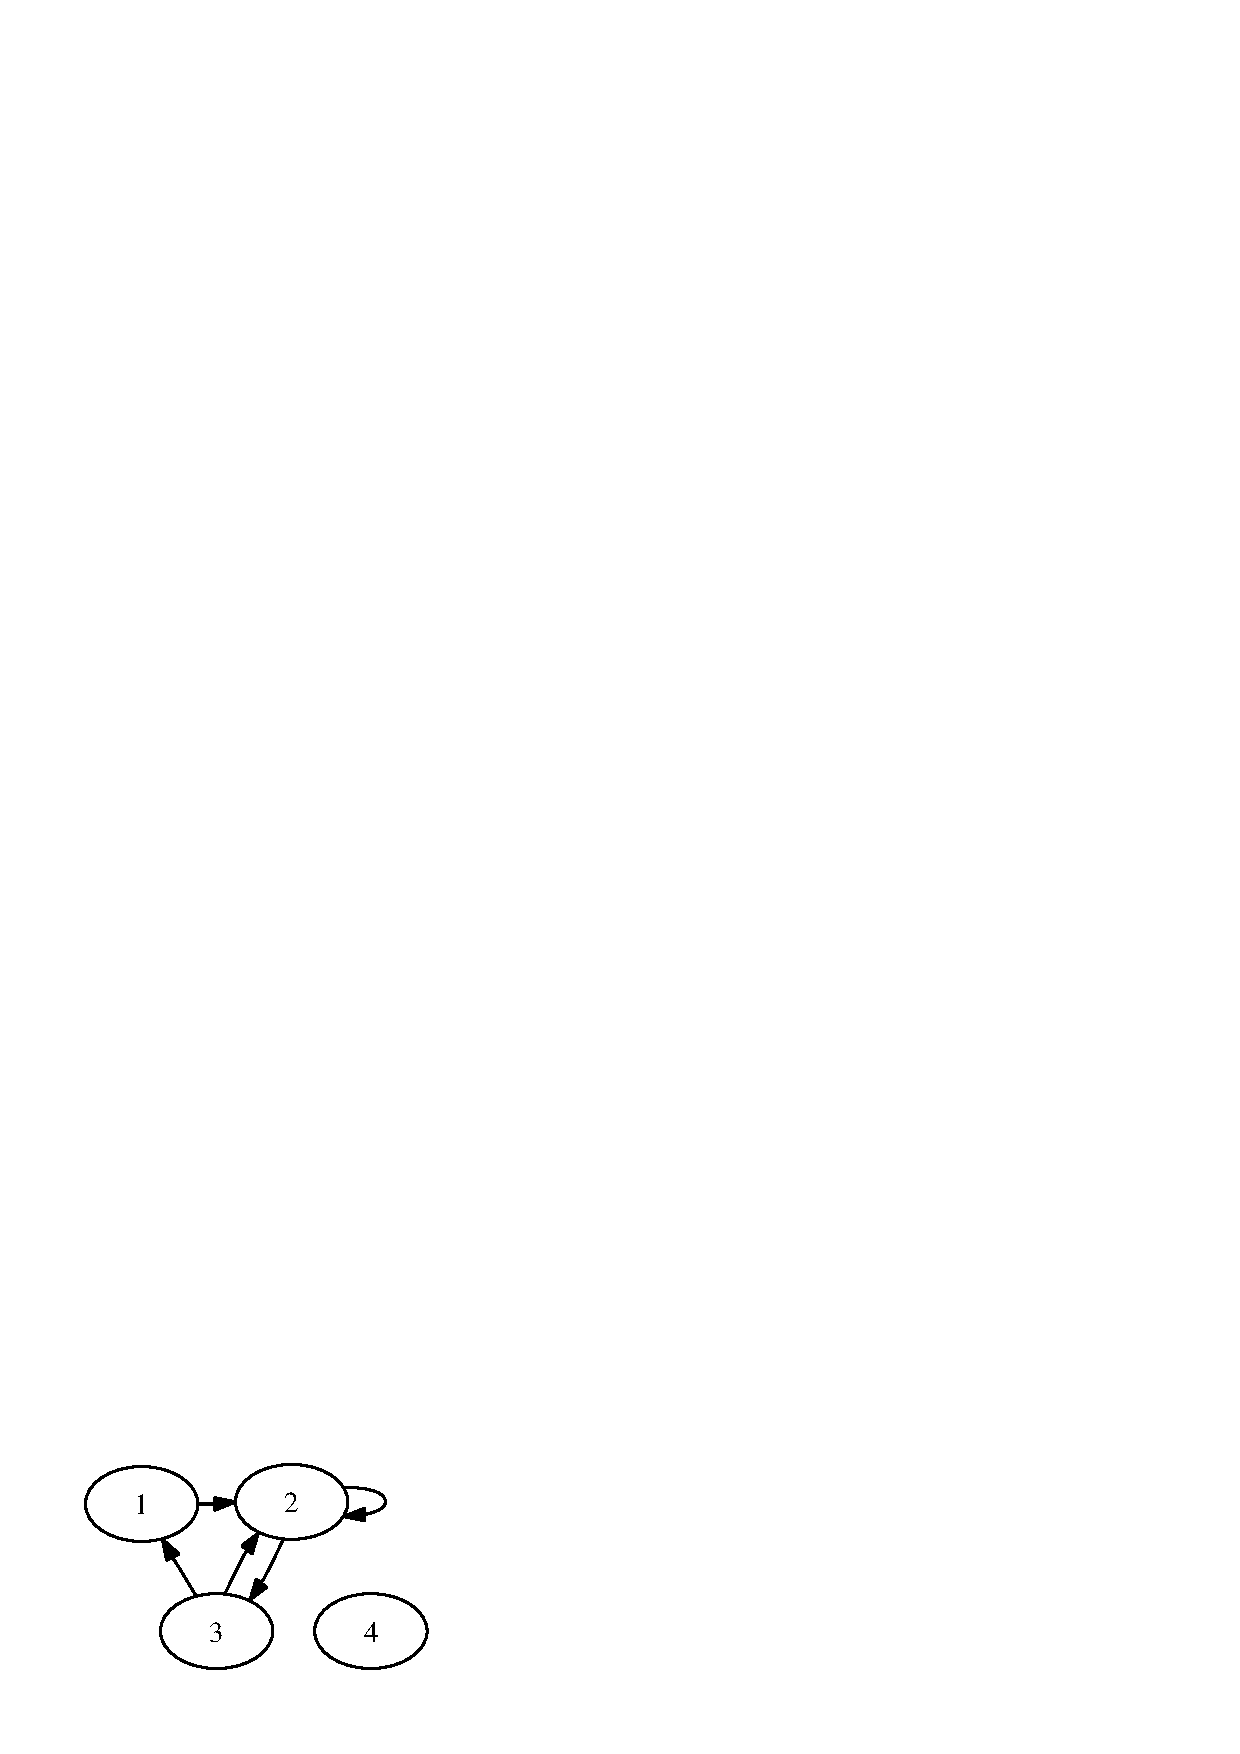
\includegraphics[width=0.4\textwidth]{digraph}
  \caption{A finite directed graph $G$}
  \label{fig:digraph}
\end{figure}
%
A common representation is a pair of lists $(\ell_V, \ell_A)$, where
$\ell_V$ is the list of vertices and $\ell_A$ the list of arrows,
known as the \emph{adjacency list}. In our example, $\ell_V = [1; 2;
3; 4]$ and $\ell_A = [(1,2); (2,2); (2,3); (3,2); (3;1)]$. Thus we
define the datatype of graphs to be\footnote{We use Ocaml notation in
  which $\clist{t}$ means lists of elements of type~$t$, and
  $t_1 * t_2$ means the type of ordered pairs whose first component
  has type $t_1$ and second type $t_2$.}
%
\begin{equation*}
  \ctype \mathtt{graph} = \clist{\cint} * \clist{(\cint * \cint)}
\end{equation*}
%
However, this is not a complete description of the representation, as
there are representation invariants and conditions which are not
expressed directly in the programming language, such as:
%
\begin{enumerate}
\item The order in which vertices and arrows are listed is not
  important, e.g., $[1;2;3;4]$ and $[4;1;2;3]$ represent the same vertices.
\item Each vertex and arrow must be listed exactly once.
\item Infinite, cyclic lists, and non-terminating values, are not
  valid representations, e.g.,
  %
  \begin{equation*}
    \cwhile{\ctrue}{()}; [(1,2);(2,2);(2,3);(3,2);(3;1)]
  \end{equation*}
  %
  is not a valid adjacency list, and neither is an expression that
  raises an exception.
\item We ought to decide which computational effects, if any, are
  allowed, e.g., is
  %
  \begin{equation*}
    \cprint{\cstring{Hello}}; [(1,2);(2,2);(2,3);(3,2);(3;1)]
  \end{equation*}
  %
  a valid adjacency list?
\end{enumerate}
%
An implementation of the set~$\mathcal{G}$ should tell us not only
what the underlying datatype $\mathtt{graph}$ is, but also which
values of type $\mathtt{graph}$ represent elements of~$\mathcal{G}$,
as well as when two such values represent the same element. As we
shall see next, all of this can be expressed by a \emph{partial
  equivalence relation}~$\per$, or \emph{per} for short, defined on
the set of values of type~$\mathtt{graph}$.

We now give the formal definition of typed realizability, as it
applies to Ocaml. Other programming languages could be used instead,
as long as they provide the usual ground types, product and function
types. Additionally, it is convenient to work with a language that
supports sum types, as this allows a more natural representation of
disjoint unions.

Let $\Type$ be the collection of all (non-parametric) Ocaml types. To
each type $t \in \Type$ we assign the set $\terminating{t}$ of
terminating values of type~$t$ which behave \emph{functionally} in the
sense of~\cite{longley99when}. Such values may not diverge, raise
exceptions or return different results on different invocations,
although they \emph{may} use exceptions, store, and other
computational effects, as long as they behave as if they did not. A
useful example of a functional value using exceptions is presented in
Section~\ref{sec:we-show-modulus-of-continuity-example}. Note also
that a terminating value of a functional type may diverge as soon as
it is applied, e.g., if we define $\cletrec{f\;x}{f\;(x+1)}$ then $f
\in \terminating{\cint \to \cint}$.

The collection $\Type$ with the assignment of terminating values $|t|$
to each $t \in \Type$ forms a \emph{typed partial combinatory algebra
  (TPCA)}. This provides a theoretical basis for the definition of a
realizability model that suits our needs. Recall that a \emph{partial
  equivalence relation} on a set~$S$ is a symmteric and transitive
binary relation on~$S$.

\begin{definition}
  A \emph{per} $A = (\typeOf{A}, {\per_A})$ is given by a type
  $\typeOf{A} \in \Type$ and a partial equivalence relation $\per_A$
  on $\terminating{\typeOf{A}}$. The \emph{support} of~$\per_A$ is the
  set $\support{A} = \set{v \in \terminating{\typeOf{A}} \such v
    \per_A v}$.
\end{definition}



\bigskip\bigskip


Outline:
%
\begin{enumerate}
\item explain how PER models are a natural semantic model for a
  programmer, because they capture ideas like
\item choice of representation and representation invariants,
\item definition of a PER model, which makes things more precise, in
  particular
\item what computational model we use (ML-like language, terminating
  values are used to represent things), and
\item what the category of PER's is (but sweep categories under the
  rug)
\item discuss relationship with ``ordinary'' realizability a la
  Kleene~\cite{KleeneSC:intint}, since logicians and theoreticians
  usually know that kind
\end{enumerate}

There ought to be some examples here.

\section{Singatures and specifications}
\label{sec:sing-spec}

Outline:
%
\begin{enumerate}
\item We introduce assertions by saying that signatures only describe a
  part of a specification
\item Our assertions talk about per's
\item They are written in the negative fragment,
\end{enumerate}


\section{The Input Language}
\label{sec:input-language}

Explain the input language and its semantics.

\section{Translation}
\label{sec:translation}

Explain the translation.




%%% Local Variables: 
%%% mode: latex
%%% TeX-master: "cie"
%%% End: 
